\chapter[Requisitos de Software]{Requisitos de Software}

\section{Introdução}\index{Introdução}
A ideia principal deste documento é reunir informações, analisar e definir necessidades a um nível superior, mais geral, do Repositório do Conhecimento da FS Desenvolvimento de Soluções de Software. Como foco, tem-se os envolvidos e usuários-alvo do sistema, bem como, suas necessidades, problemas e as razões que dão corpo a essas necessidades. Detalhes de como serão sanados os problemas e como serão trabalhados, serão feitos em formato de User Stories.

\subsection{Finalidade}\index{Finalidade}
O presente documento possui como objetivo realizar a execução do processo de engenharia de requisitos que contém: atividades,  papéis, responsabilidades e artefatos, que já foram previamente descritos no primeiro trabalho da disciplina de requisitos de software. 
Além disso o sistema proposto neste relatório destina-se à automação de uma  solução que auxilie na disposição de informações para problemas e soluções de projetos realizados pela equipe da FS desenvolvimento de soluções de software.

\subsection{Escopo}\index{Escopo}
Este relatório dá uma visão geral do que foi trabalhado no que tange à definição dos requisitos de software para a empresa FS Desenvolvimento de Software. Nele, serão abordados o escopo do produto, descrição do problema, o tema de investimento, épicos, features, histórias de usuário, critérios de aceitação, processo de Engenharia de Requisitos, Roadmap, Requisitos não funcionais, restrições do produto, análise de problemas e necessidades da empresa, definição e detalhamento dos requisitos e técnicas utilizadas, restrições de qualidade do produto, rastreabilidade, usuários, envolvidos, planejamento da equipe e lições aprendidas durante o projeto, seguindo ao processo que foi definido no primeiro trabalho. 

\section{Técnicas de Elicitação}\index{Técnicas de Elicitação}
A princípio ficou decidido a utilização de duas técnicas: entrevista e workshop, para a elicitação dos requisitos porém o grupo sentiu a necessidade de utililizar a técnica de prototipação, além das que foram propostas.

\subsection{Entrevista}\index{Entrevista}
Técnica escolhida principalmente pela eficiência, velocidade de seu retorno e pela facilidade que a equipe teria de conduzir uma entrevista, visto que a equipe se encontrava semanalmente, com todos os integrantes da equipe presentes, teve início uma conversa informal de como a organização FS Soluções de Software trabalhava, como lidava com problemas, e no decorrer desta conversa foram percebidas algumas outras dificuldades que a empresa enfrentava, que provavelmente, por outros métodos seriam mais custosos de se enxergar, apenas com a entrevista, a equipe de requisitos teve uma ideia inicial de como os problemas aconteciam, mas para fixação da ideia, foi feito um brainstorm com o propósito de clarear a percepção a respeito das necessidades dos clientes, ainda na presença dos clientes, foram feitos desenhos no quadro negro de como o sistema teria que se comportar, e o que ele teria de fazer, para sanar os problemas da organização, e os clientes, validavam ou não as ideias que eram apresentadas, incrementando assim, a técnica de prototipação para a elicitação de requisitos.
Para a entrevista foram levantadas as seguintes perguntas:
\begin{itemize}
\item Quantas pessoas trabalham em um projeto?
\item Essas pessoas tem papeis diferentes, ou todos fazem as mesmas coisas?
\item Todos tem visibilidade do que cada um está fazendo?
\item Quais as situações que estressam, ou atrapalham a equipe durante o projeto?
\item Quando um funcionário sai da equipe, tem-se alguma forma de registro do que ele fez e do que ele estava fazendo?
\item Todos podem gerar relatórios de entrega para os clientes?
\item Esses relatórios são gerados somente quando requisitados, ou deve ter um controle mesmo quando o cliente não pede?
\end{itemize}

\subsection{Workshop}\index{Workshop}
Workshop trata como a equipe apresenta novas ideias e soluções que teriam de ser validadas pelo cliente, onde, portando formas mais bem construídas  da solução parcial e próximas a verdadeira face do sistema, teriam o aval do público-alvo, se aquilo que estava sendo pensado seria bem aceito e podendo assim dar continuidade a construção, sempre alinhado com as vontades dos clientes.

\subsection{Prototipação}\index{Workshop}
A prototipação foi utilizada como uma forma de entender os problemas dos clientes, foi feita a partir de uma brainstorm, a equipe deixou claro que aquilo não seria como o sistema se pareceria, e que aquelas ideias eram somente para auxiliar no entendimento do contexto, pois eram apenas ideias tomando uma forma mais crua, para poder dar corpo a um sistema mais elaborado. Em um primeiro momento, a prototipação estava sendo feita antes da criação das história de usuário mas, após a orientação do professor, os protótipos foram descartados e foram refeitos após a criação das histórias com o intuito de criar os critérios de aceitação. O protótipo foi criado utilizando a ferramenta Balsamiq que foi escolhida devida a familiaridade da equipe com a ferramenta. Em anexo está a versão final do protótipo que foi utilizada pela equipe.

\section{Posicionamento}\index{Posicionamento}
Este tópico apresenta a oportunidade de negócio da empresa, o problema que a empresa está enfrentando, a proposta de um produto que atenda as necessidades da empresa e o tema de investimento que é a área onde a empresa quer investir.

\subsection{Oportunidade de Negócios}\index{Oportunidade de Negócios}
A empresa FS Desenvolvimento de Soluções de Software atua no mercado de desenvolvimento de software e está passando  por dificuldade na gestão de informações. Por exemplo: se ocorre à substituição de  membros  a  equipe costuma perder o histórico de atividades da pessoa que saiu da equipe, bem como suas soluções dadas às questões do projeto. Além disso quando um cliente pede um relatório para saber do andamento do projeto , a equipe perde tempo confeccionando o mesmo. Observando o cenário atual, a direção da FS deseja identificar e melhorar os processos mais críticos da empresa.

\subsection{Tema de Investimento}\index{Tema de Investimento}
Para o caso da FS Software, o Tema de Investimento identificado foi o Gerenciamento de informações da empresa. Que diz respeito ao controle e monitoramento das atividades realizadas por cada membro da equipe durante a execução dos projetos realizados na empresa FS desenvolvimento de soluções de software.

\subsection{Descrição do Problema}\index{Descrição do Problema}
Uma  forma para abordar o problema, subproblemas e possíveis soluções  é criando um framework. A tabela  apresentada abaixa mostra o problema, subproblema e sugestão de solução encontrada pela equipe:

\begin{table}[H]
\caption{Framework de Descrição do Problema.}
\centering
\begin{tabular}{ | p{3cm} | p{9cm}| }
\hline
\textbf{O problema de} & Falta de disseminação do conhecimento.\\ \hline
\textbf{afeta} & Os integrantes da equipe. \\ \hline
\textbf{cujo impacto é} & Stress  na geração dos relatórios e atraso no comprometimento dos prazos e perda do conhecimento. \\ \hline
\textbf{uma boa solução seria} & Arquivar e disponibilizar conhecimento. A criação de um registro das atividades de trabalho, facilitaria na geração de relatório e daria  visibilidade do projeto ao cliente sem gerar stress na equipe. \\ \hline
\end{tabular}
\end{table}

\subsection{Diagrama de causa e efeito}\index{Diagrama de causa e efeito}
O Diagrama de causa e efeito , que também é conhecido como “ Fishbone” é uma maneira de esquematizar um problema e suas respectivas causas. Ele possui como objetivo facilitar a visualização das causas e problema que foram encontrados em um determinado contexto.
O grupo fez e refez diversos “Fishbones” durante a realização desse segundo trabalho, e pelas conversas de validação realizadas com o professor o grupo chegou a um diagrama final que está representado na figura 1.\\

\begin{figure}[H]
\centering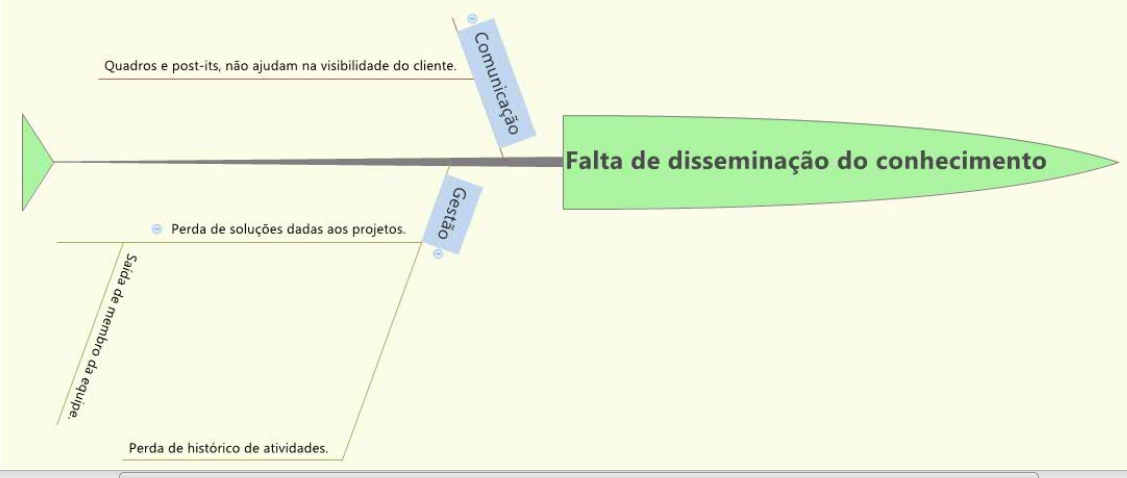
\includegraphics[scale=0.5]{figuras/fishbone.png}
\caption{\textit{Diagrama Causa-Efeito do Problema.}}
\end{figure}


\subsection{Sentença de Posição do Produto}\index{Sentença de Posição do Produto}
\begin{table}[H]
\caption{Sentença de Posição do Produto}
\centering
\begin{tabular}{ | p{3cm} | p{9cm}| }
\hline
\textbf{Para} & A FS Desenvolvimento de Soluções de Software\\ \hline
\textbf{Que} & Necessita de uma solução para gerenciamento de informações da empresa \\ \hline
\textbf{O Repositório do Conhecimento} & É um  gerenciador de informações \\ \hline
\textbf{Que} & 1 - Mostra uma visibilidade das informações dos projetos bem como arquiva e as controla, faz o gerenciamento do conhecimento individual de cada integrante da equipe, que posta um problema em um quadro de problemas ou uma solução de um problema de outro integrante da equipe e cria um portfólio de tecnologias utilizadas na empresa que incluem, entre outras funções, usos indicados de uma determinada tecnologia, especialistas dentro da equipe nessa tecnologia e suas principais referências.
 \\ \hline
 \textbf{Diferente de} & Planilhas de excel e conversas informais em grupos de rede social\\ \hline
 \textbf{Nosso produto} & Nosso produto tem todas as funcionalidades para gestão de conhecimento e tecnologias utilizadas centralizadas em um único produto, que requer menos tempo e esforço por parte da equipe para preenchimento das informações\\ \hline
\end{tabular}
\end{table}

\section{Descrições dos Usuários}\index{Descrições dos Usuários}
A FS Desenvolvimento de Soluções de Software trabalha atualmente com equipes pequenas para a produção de software. Os funcionários da empresa possuem alto conhecimento em todas as áreas da engenharia de software permitindo assim a rotatividade de funções entre os integrantes da equipe, uma vez que, para cada projeto, um membro executa uma função apenas. As funções são dividas em desenvolvedor, analista de requisitos, arquiteto, testador e gerente de projeto. Além dessas funções, existe a função de Gerente do Conhecimento que não é rotacionada entre projetos, dado que a gerência do conhecimento é feita para toda a empresa e não para projetos específicos.

\subsection{Resumo dos Usuários}\index{Resumo dos Usuários}

\begin{table}[H]
\caption{Resumo dos Usuário}
\centering
\begin{tabular}{ | p{3cm} | p{5cm}| p{5cm} | }
\hline
\textbf{Nome} & Descrição & Responsabilidades \\ \hline
\textbf{Gerente Geral} & Responsável pelo gerenciamento dos projetos da empresa. & Registra novos usuários, aloca usuários em projetos e registra novos projetos \\ \hline
\textbf{Gerente do Conhecimento} & Responsável pelo gerenciamento do conhecimento da empresa. & Manter portfólios de conhecimento \\ \hline
\textbf{Desenvolvedor} & Responsável pela codificação dos projetos da empresa. & Registrar suas atividades, registrar problemas e registrar soluções \\ \hline
\textbf{Testador} & Responsável pelos testes dos códigos da empresa. & Registrar suas atividades, registrar problemas e registrar soluções \\ \hline
\textbf{Analista de Requisitos} & Responsável pelo levantamento dos requisitos da empresa. & Registrar suas atividades, registrar problemas e registrar soluções \\ \hline
\textbf{Arquiteto} & Responsável pela arquitetura dos sistemas que a empresa desenvolve. & Registrar suas atividades, registrar problemas e registrar soluções \\ \hline
\end{tabular}
\end{table}

\section{Visão Geral do Produto}\index{Visão Geral do Produto}

\subsection{Perspectiva do Produto}\index{Perspectiva do Produto}
O Repositório do Conhecimento faz com que o acompanhamento do trabalho da equipe e a gerência do conhecimento da equipe seja realizado com maior facilidade. Com o software, o usuário registrará tudo que está fazendo bem como suas dificuldades, além de poder auxiliar outro usuário com as dificuldades dele. Além disso, o usuário poderá ver um portfólio de tecnologia que mostra o que a empresa sabe sobre determinada tecnologia, assim como seus problemas encontrados e soluções. Com essas informações, são gerados relatórios que aumentam a visibilidade do cliente da FS Software sobre o projeto.

\section{Requisitos funcionais}\index{Requisitos funcionais}

\subsection{Épicos}\index{Épicos}
Os épicos identificados foram:
\begin{itemize}
\item \textbf{Épico 1 - Informações dos projetos} - Que diz respeito a visibilidade, arquivamento e controle das informações que são cadastradas pelos membros da equipe de trabalho. 
\item \textbf{Épico 2 - Informações de recursos humanos} - Este épico refere-se a gerencia do conhecimento que cada integrante da equipe possui e a manutenção do portifólio de informações.
\end{itemize}

\subsection{Features}\index{Features}
As features levantandas foram:
\begin{itemize}
\item \textbf{Feature 1- Visibilidade das informações dos projetos (Épico 1)}
\item \textbf{Feature 2- Arquivamento das informações (Épico 1)}
\item \textbf{Feature 3- Controle das informações (Épico 1)}
\item \textbf{Feature 4- Gerenciamento do conhecimento individual (Épico 2)}
\item \textbf{Feature 5- Manutenção do portfólio (Épico 2)}
\end{itemize}

\subsection{Histórias de Usuário}\index{Histórias de Usuário}
As histórias de usuário para o Repositório do Conhecimento são:
\begin{itemize}
\item \textbf{US1 - Eu, como gerente de projeto desejo gerar relatório, para que eu possa fazer um documento de acompanhamento que será disponibilizado aos clientes da empresa quando solicitado. (Feature 1)}
\item \textbf{US2 - Eu, como gerente do projeto desejo visualizar as horas gastas ,dos funcionários em cada atividade, para que eu possa ter um controle da produtividade de cada membro da equipe. (Feature 1)}
\item \textbf{US3 - Eu, como integrante da equipe desejo me comunicar com outros integrantes do projeto que participo por meio de chat em suas atualizações, para que eu possa discutir sobre seus registros de trabalho. (Feature 2)}
\item \textbf{US4 - Eu, como usuário, desejo editar os meus registros de atividades para atualizar o que foi trabalhado. (Feature 2)}
\item \textbf{US5 - Eu, como integrante da equipe, desejo registrar as atividades que estou desempenhando para que fique visível aos outros integrantes do projeto. (Feature 2)}
\item \textbf{US6 - Eu, como gerente, desejo remover o acesso de determinado usuário para que ele não tenha possibilidade de entrar no sistema. (Feature 3)}
\item \textbf{US7 - Eu, como gerente do projeto desejo incluir integrantes da equipe em perfis de usuário, para que cada integrante tenha acesso às informações que digam respeito a somente seu perfil de usuário. (Feature 3)}
\item \textbf{US8 - Eu, como integrante da equipe, desejo editar as informações cadastrais no sistema, para atualizar meus dados pessoais e as tecnologias que domino. (Feature 3)}
\item \textbf{US9 - Eu, como integrante da equipe, desejo visualizar a lista de problemas para contribuir com soluções. (Feature 4)}
\item \textbf{US10 - Eu, como integrante da equipe, desejo encontrar soluções por meio dos problemas já cadastrados para solucionar o meu problema. (Feature 4)}
\item \textbf{US11 - Eu, como integrante da equipe, desejo dar soluções de problemas cadastrados por outros colegas, para que eles possam solucionar seus problemas e prosseguir com o andamento do projeto. (Feature 4)}
\item \textbf{US12 - Eu, como integrante da equipe, desejo cadastrar informações de problemas que estou tendo ao decorrer do projeto, para que outros integrantes possam me ajudar com soluções que eles possam conhecer. (Feature 4)}
\item \textbf{US13 - Eu, como gerente de conhecimento, desejo editar os portfólios de tecnologias disponíveis para que os portfólios estejam mais corretos em relação a informação e redação. (Feature 5)}
\item \textbf{US14 - Eu, como gerente de conhecimento, desejo criar uma categoria de portfólio de tecnologias para que os portfólios fiquem melhor organizado. (Feature 5)}
\item \textbf{US15 - Eu, como gerente de conhecimento, desejo cadastrar em uma categoria do portfólio uma determinada tecnologia e seu especialista, sugestão de uso, referências e projetos que já tenha utilizado essa tecnologia, para que usuários possam ter uma informação de ajuda sobre a tecnologia. (Feature 5)}
\item \textbf{US16 - Eu, como gerente do conhecimento, desejo disponibilizar um portfólio de tecnologias utilizadas na empresa, para que a equipe  tenha um material de apoio que os auxiliem no conhecimento de determinada tecnologia. (Feature 5)}
\end{itemize}

\subsection{Matriz de Rastreabilidade de Requisitos Funcionais}

As figuras a seguir mostram a rastreabilidade dos requisitos funcionais que foram geradas pela ferramenta Caliber.

Utilizando a ferramenta Caliber foram gerados matrizes de rastreabilidade, que auxiliam no acompanhamento de itens de importância para o projeto, tem-se  a matriz de Épicos e Features, mostrando de onde cada Feature saiu, tornando a consulta mais instintiva e fácil.

\begin{figure}[H]
\centering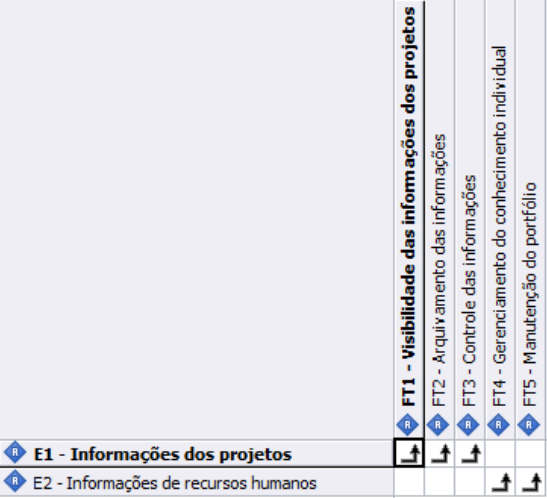
\includegraphics[scale=0.5]{figuras/rastreabilidade1.png}
\caption{\textit{Matriz de Rastreabilidade de Épicos x Features utilizando a ferramenta Caliber}}
\end{figure}

Nesta próxima matriz, podemos ver a relação entre features e histórias de usuário, caso seja necessária a consulta, esta matriz mostra de maneira mais transparente tais relacionamentos.

\begin{figure}[H]
\centering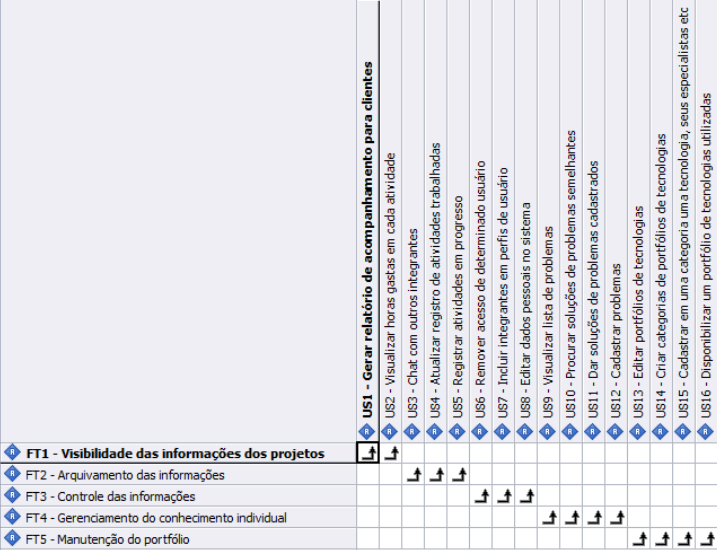
\includegraphics[scale=0.5]{figuras/rastreabilidade2.png}
\caption{\textit{Matriz de Rastreabilidade de Features x Histórias de Usuário utilizando a ferramenta Caliber}}
\end{figure}

Matriz que mostra a relação entre épicos e histórias de usuário, aumentando a visibilidade da relação entre tais itens. 

\begin{figure}[H]
\centering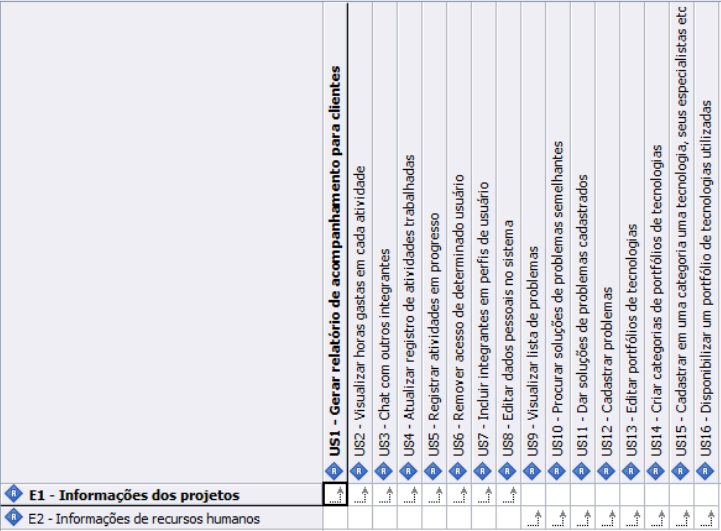
\includegraphics[scale=0.5]{figuras/rastreabilidade3.png}
\caption{\textit{Matriz de Rastreabilidade de Épicos x Histórias de Usuário implicadas nos épicos utilizando a ferramenta Caliber}}
\end{figure}

\subsection{Critérios de Aceitação}\index{Critérios de Aceitação}
Para a estruturação dos critérios, foi utilizado o template do BDD. Para a primeira release, foi priorizada a feature 4 (Gerenciamento do conhecimento individual). Para as histórias desta feature, foram levantados os seguintes critérios de aceitação:

\textbf{US9. Eu, como integrante da equipe, desejo visualizar a lista de problemas para contribuir com soluções.}

\textbf{Cenário 1: Buscar problemas sem solução}
Dado uma busca por problemas\\
Então são opcionais os filtros:  
\begin{itemize}
\item Tipo de Tecnologia
\item Problema sem Solução (status)
\item Texto (descrição do problema)
\end{itemize} 

\textbf{Cenário 2: Abrir detalhes do problema}
Dado um problema encontrado\\
Quando o registro for clicado\\
Então é aberto um detalhamento do problema\\

\textbf{US10. Eu, como integrante da equipe, desejo encontrar soluções por meio dos problemas já cadastrados para solucionar o meu problema.}

\textbf{Cenário 1: Buscar soluções}
Dado uma busca por soluções\\
Então são opcionais os filtros:
\begin{itemize}
\item Tipo de Tecnologia
\item Texto (descrição do problema)
\end{itemize} 

\textbf{Cenário 2: Abrir descrições das soluções}
Dado um problema já solucionado encontrado\\
Quando o registro do problema é clicado\\
Então é aberto uma lista de descrições das soluções\\

\textbf{US11. Eu, como integrante da equipe, desejo dar soluções de problemas cadastrados por outros colegas, para que eles possam solucionar seus problemas e prosseguir com o andamento do projeto.}

\textbf{Cenário 1: Problema já criado}
Dado um problema que já foi criado\\
Então apenas o autor e o gerente do conhecimento pode editar e deve ficar visível para todos que o problema foi editado\\

\textbf{Cenário 2: Problema com solução}
Dado um problema já solucionado\\
Então podem existir mais de uma solução para cada problema\\

\textbf{Cenário 3: Problema com solução sem marcação}
Dado um problema com uma solução\\
Então o autor pode marcar o problema como resolvido\\

\textbf{US12. Eu, como integrante da equipe, desejo cadastrar informações de problemas que estou tendo ao decorrer do projeto, para que outros integrantes possam me ajudar com soluções que eles possam conhecer.}

\textbf{Cenário 1: Pesquisar problema cadastrado}
Dado um problema a ser cadastrado\\
Então é necessário que seja feita uma pesquisa para não repetir problemas\\

\textbf{Cenário 2: Cadastrar problema}
Dado um problema a ser cadastrado\\
Então são necessárias as seguintes informações:
\begin{itemize}
\item Título do Problema
\item Tecnologia associada
\item Detalhes do problema
\end{itemize} 

\section{Restrições}\index{Restrições}
Do ponto de vista de usuários, sem permissões de administrador, não se pode ter visibilidade de informações pessoais, postar com outro nome, modificar, excluir ou adicionar outras contas.

\section{Requisitos não Funcionais}\index{Requisitos não Funcionais}

\subsection{Implementação}\index{Implementação}
O sistema deverá ser criado utilizando a ferramenta Bizagi Studio.

\subsection{Confiabilidade}\index{Confiabilidade}
O sistema deverá ficar disponível 24 horas por dia, 7 dias por semana sem exceções.

\subsection{Suportabilidade}\index{Suportabilidade}
O sistema pode ser acessado através dos navegadores Chrome (versão 38.0.2125.11 ou posterior),  Mozilla  Firefox (versão 33.1.1 ou superior),  Safari (versão 5.1.7 ou superior) e Internet Explorer (versão 11 ou superior).

\subsection{Desempenho}\index{Desempenho}
O sistema deve fazer uma atualização com tempo inferior ou igual a 2 segundos.

\subsection{Portabilidade}\index{Portabilidade}
O sistema deve funcionar, nos sistemas operacionais Linux, e Windows.\\
O sistema deve ser ajustável a visão mobile.

\section{Requisitos de Documentação}\index{Requisitos de Documentação}

\subsection{Manual do Usuário}\index{Manual do Usuário}
O manual do usuário deverá ser impresso em papel tamanho A5, fornecendo detalhes de cada função do sistema, como: a finalidade da função e os passos para realizar uma ação em determinada função, bem como um exemplo prático da função se for possível. O manual deverá conter um índice no início do documento e um índice remissivo ao final do documento contendo os assuntos tratados em cada página. Deverá conter também um glossário de termos utilizados no manul dispostos em ordem alfabética. O texto do manual do usuário deverá ser escrito em fonte Arial nos seguintes tamanhos e formatos:
\begin{itemize}
\item Títulos e subtítulos: fonte tamanho 10 em negrito;
\item Conteúdo: fonte tamanho 9 não-negrito.
\end{itemize} 
O texto deverá estar justificado na página e com margens - tanto superior e inferior, quanto laterais - espaçadas em 1,5cm.

\subsection{Ajuda On-line}\index{Ajuda On-line}
Deverá existir uma página para ajuda On-line com soluções de problemas frequentes (FAQ), telefones de contato da equipe de suporte bem como uma área para chat com atendentes para soluções de dúvidas não encontradas na página e uma área para atendimento por e-mail para contato quando não houver disponibilidade de chat.

\subsection{Guias de Instalação e de Configuração, e Arquivo Leia-me}\index{Guias de Instalação e de Configuração, e Arquivo Leia-me}
Como a solução será implementada em padrão web, deverá portanto haver uma sessão na página da aplicação contendo instruções de instalação, configuração, requisitos mínimos do sistema a ser usado e plugins adicionais a serem utilizados.

\section{Planejamento das Sprints}\index{Planejamento das Sprints}
\subsection{1ª Sprint}\index{1ª Sprint}
Na 1ª Sprint, foram planejadas as seguintes histórias de usuário da Feature 4 (F4), compondo assim a Release 1:
\begin{itemize}
\item US9 - Eu, como integrante da equipe, desejo visualizar a lista de problemas para contribuir com soluções.
\item US10 - Eu, como integrante da equipe, desejo encontrar soluções por meio dos problemas já cadastrados para solucionar o meu problema.
\item US11 - Eu, como integrante da equipe, desejo dar soluções de problemas cadastrados por outros colegas, para que eles possam solucionar seus problemas e prosseguir com o andamento do projeto.
\item US12 - Eu, como integrante da equipe, desejo cadastrar informações de problemas que estou tendo ao decorrer do projeto, para que outros integrantes possam me ajudar com soluções que eles possam conhecer.
\end{itemize}

\section{Roadmap}\index{Roadmap}
O projeto foi dividido em 3 releases. Para a primeira release do projeto, foi priorizada a feature 4(Gerenciamento do conhecimento individual) pois esta contém as funcionalidades mais importantes para o cliente em um primeiro momento. Na segunda release, as features 2(Arquivamento das informações) e 3(Controle das informações) geram bastante valor ao auxiliar no gerenciamento das informações do projeto que não é contemplado na primeira release e uma feature complementa a outra. As features 1 e 5 foram alocadas para a última release. A figura 3 demonstra melhor como foram divididas as features.\\

\begin{figure}[H]
\centering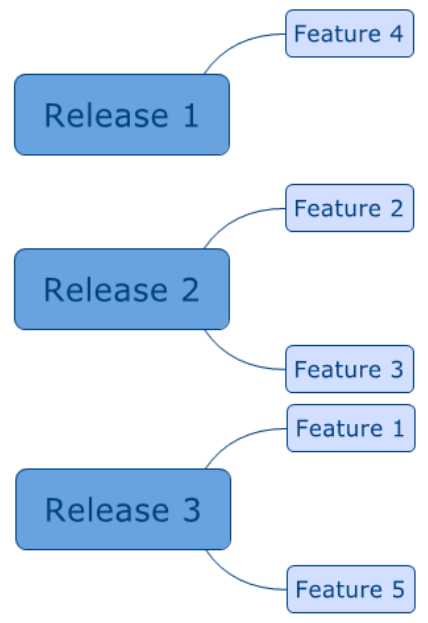
\includegraphics[scale=0.5]{figuras/roadmap.png}
\caption{\textit{Roadmap do Repositório do Conhecimento.}}
\end{figure}

\section{Processo de ER}\index{Processo de ER}
Na primeira entrega, foi proposto um processo de engenharia de requisitos que visava a metodologia escolhida. Conforme o processo foi sendo executado, foram observadas que algumas mudanças seriam necessárias para a melhor realização do trabalho. O processo modelado no Bizagi que foi utilizado pela equipe é encontrado no final deste documento no apêndice  E . As atividades que sofreram mudanças foram: Elicitar Requisitos, Detalhar Requisitos e Atualizar Backlog do Produto a qual foi inserida no processo. Na atividade Elicitar Requisitos, eram artefatos de saída: o Visão e o Backlog do Produto. Porém como foi necessário fazer a validação parcial do Visão ao invés de redigir o documento na íntegra e só depois validar, o modelo foi alterado para que a saída do Elicitar Requisitos fosse o Visão parcial e após as validações era verificado se o documento estava completo antes de seguir em frente.  Na atividade Detalhar Requisitos, foi inserido o artefato Protótipo. A atividade de Fazer Protótipo foi inicialmente feita em um momento não apropriado e, após a orientação do professor, foi refeita no momento correto. 

\section{Cronograma}\index{Cronograma}

Na iteração 2, na disciplina de Planejamento fizemos as atividades de Realizar entrevista com clientes, Criar fishbone do sistema, Identificar requisitos não funcionais, Validar requisitos não funcionais, Identificar user stories, Modelar protótipo, Validar Tema de investimento e Documentar os itens identificados e validados.

Já na atividade de Execução na iteração 2 foram desempenhadas as atividades de Priorizar user stories para a 1ª Sprint, validar user stories, Detalhar user stories priorizadas, registrar os requisitos e rastreabilidade na ferramenta de gerenciamento de requisitos e os pontos de controle com o professor.

Quanto as mudanças ocorridas desde a primeira versão, seguem na tabela abaixo as atividades com alteração e suas respectivas alterações

\textbf{Planejamento}
\begin{table}[H]
\caption{Tabela de mudanças na disciplina de Planejamento}
\centering
\begin{tabular}{ | p{3cm} | p{9cm}| }
\hline
\textbf{Atividade } & \textbf{Mudança(s)}\\ \hline
Entrevista com os clientes & Inclusão \\ \hline
Criar fishbone do sistema & Alteração de data final para 13/11/2014 \\ \hline
Identificar temas de investimento, épicos e features & Alteração de data inicial para 05/11/2014 e final para 11/11/2014 \\ \hline
Identificar requisitos não funcionais & Alteração de data inicial para 05/11/2014 e final para 13/11/2014\\ \hline
Validar requisitos não funcionais & Inclusão\\ \hline
Identificar user stories & Alteração de data inicial para 11/11/2014 e final para 12/11/2014 \\ \hline
Modelar protótipo & Inclusão\\ \hline
Validar Tema de investimento, épicos e features & Alteração de data inicial para 12/11/2014 e final para 12/11/2014\\ \hline
Documentar os itens identificados e validados & Alteração de data inicial para 12/11/2014 e final para 20/11/2014SSS\\ \hline
\end{tabular}
\end{table}

\textbf{Execução}
\begin{table}[H]
\caption{Tabela de mudanças na disciplina de Execução}
\centering
\begin{tabular}{ | p{3cm} | p{9cm}| }
\hline
\textbf{Atividade } & \textbf{Mudança(s)}\\ \hline
Priorizar user stories para 1ª sprint & Alteração de data inicial para 17/11/2014 e final para 17/11/2014 \\ \hline
Validar users stories & Alteração de data inicial para 13/11/2014 e final para 17/11/2014 \\ \hline
Detalhar user stories priorizados & Alteração de data inicial para 21/11/2014 e final para 01/12/2014\\ \hline
Registrar requisitos e rastreabilidade na ferramenta de GR & Alteração de data inicial para 01/12/2014 e final para 03/12/2014\\ \hline
Apresentação do trabalho 2 & Alteração de horário inicial para 9:00 \\ \hline
\end{tabular}
\end{table}

O cronograma completo encontra-se no apêndice D.

\section{Relato de Experiência}\index{Relato de Experiência}
Este tópico aborda as experiências dos membros da equipe da disciplina de Requisitos de software e Modelagem de Processo, ministradas na universidade de Brasília, campus Gama,  durante a realização dos trabalhos ocorridos no segundo semestre de dois mil e quatorze.

As duas disciplinas possuiam  o mesmo contexto de trabalho porém cada uma tinha funções diferentes, os alunos de modelagem eram responsáveis pelo entendimento do negócio, identificação e realização de melhorias enquanto os alunos de requisitos tinham como responsabilidade elicitar e detalhar os requisitos do software e modelar o processo de ER. Os alunos de requisitos e modelagem tinham como compromisso fazer  a  automatização da solução proposta pela equipe juntos.

Foi a primeira vez que as disciplinas de Requisitos de Software e Modelagem de Processos foram ministradas juntas. Por esse fato existiram muitas dúvidas por parte dos alunos, que muitas vezes ficavam confusos em relação ao que deveria ser feito e como o trabalho seria melhor estruturado tendo em vista que não existia um documento que o grupo pudesse usar como exemplo. Durante o decorrer do trabalho também ficou confuso em alguns momentos quem era o cliente de quem  era contratado.

No que se refere as aulas de requisitos, elas foram produtivas pois o professor tem experiência nos conteúdos que foram apresentados e mesmo nos dias que a turma estava dispersa ele buscava a participação de todos os alunos durante as aulas. Nos   dias de aulas em que foram debatidos  os artigos que estavam  disponibilizados via moodle foi interessante as discussões levantadas. A competição realizada antes da primeira prova foi muito boa, pois foi como se fosse uma revisão de conteúdo. 

\subsection{Interação entre a equipe de Requisitos de Software}\index{Interação entre a equipe de Requisitos de Software}
Durante a execução do primeiro trabalho foi difícil o entendimento entre as partes da equipe. Dois integrantes da equipe já se conheciam, porém o outro membro nunca tinha feito trabalho com os dois. A falta de comunicação e desinteresse por parte de um dos membros da equipe fizeram com que houvesse desgaste e stress durante a realização do primeiro trabalho. O professor ficou a par da situação da equipe e realizou uma reunião entre os integrantes do grupo, depois dessa reunião a convivência e comunicação entre os membros da equipe foi totalmente diferente. Talvez se esta conversa tivesse acontecido em um momento anterior, o desgaste e o stress teriam sido evitados.

Depois da apresentação, acolhemos um novo integrante ao nosso grupo, pois o seu grupo foi dissolvido e aconteceu a realocação de um aluno para cada equipe. Não houve nenhum problema com a adição de mais um membro, todos se entenderam muito bem, e as tarefas foram realizadas em equipe de maneira clara para todos. Não existiu nenhum desentendimento e nenhuma falta de comunicação entre os integrantes do grupo nesta segunda parte do trabalho.

Do ponto de vista do novo integrante, o processo de integração com um grupo já consolidado foi em geral bem tranquilo. O grupo foi bem atencioso quando o novo integrante tinha dúvidas e considerava a opinião do mesmo como qualquer outra.

\subsection{Integração entre as equipes}\index{Integração entre as equipes}
Com relação a interação entre as equipes de Requisitos de Software e Modelagem de Processo, sempre foi boa a relação  entre essas duas equipes. Existiam conflitos de horários, mas sempre existiram encontros fixos nas segundas-feiras e quando necessário eram marcados encontros durante a semana e nos finais de semana também. A equipe de Modelagem  sempre se prontificou a ajudar, na medida do que era permitido, a equipe de Requisitos. 

Na segunda parte do trabalho,  a equipe de Modelagem também foi acrescida de mais um membro na sua equipe e isso não interferiu na boa relação que já existia no grupo. Durante as reuniões na maioria das vezes todos os integrantes estavam presentes e sempre existiu uma boa comunicação entre os grupos, isso era refletido no fato de que as equipes estavam a par do que a outra equipe estava fazendo.

\subsection{Sugestão de Melhorias}\index{Sugestão de Melhorias}
\begin{itemize}
\item É importante definir de maneira clara o papel de cada equipe na realização do trabalho, onde, os alunos sabem até ondem podem influenciar no contexto passado pelo professor.
\item Templates de relatórios auxiliariam as equipes na hora de estruturar seus trabalhos.
\item Definir de maneira mais clara como deve ser a relação entre as equipes.
\end{itemize} 

\subsection{Lições aprendidas}\index{Lições aprendidas}
Em um ambiente de trabalho, as pessoas não precisam ter afinidade para poder trabalharem juntas. Deve existir respeito por parte de todos os integrantes de uma equipe, e cada um deve se comprometer a realizar suas tarefas impostas e justificar o motivo pelo qual não fez, quando não realizadas. 

